
\begin{figure}
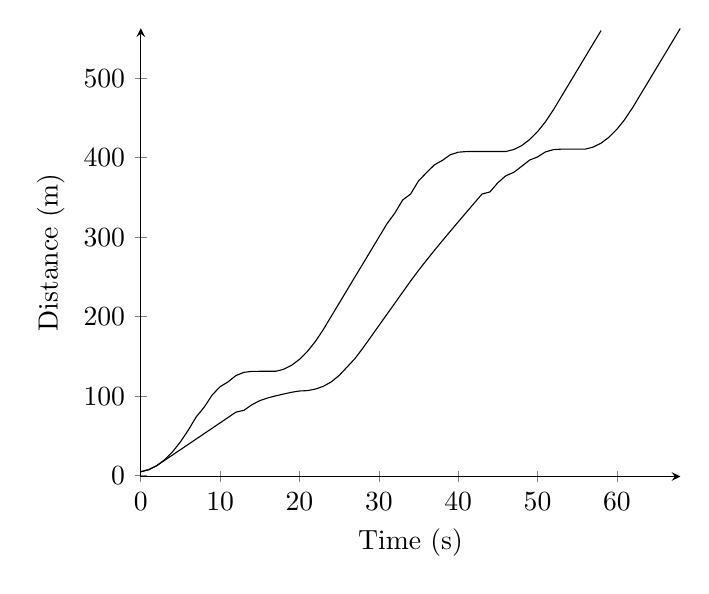
\begin{tikzpicture}
\begin{axis}[
legend style={anchor=west},
axis x line=bottom,
axis y line=left,
ymin=-1,
xlabel=Time (s),
ylabel=Distance (m),
]
\addplot[] coordinates {
(0, 5.1)
(1, 7.6)
(2, 12.6)
(3, 19.340953082)
(4, 26.0822228597)
(5, 32.8238691159)
(6, 39.5659677207)
(7, 46.3086164451)
(8, 53.0519434996)
(9, 59.7961204194)
(10, 66.5413821245)
(11, 73.288059319)
(12, 80.0366331511)
(13, 82.3278324253)
(14, 89.2955672227)
(15, 94.4741483261)
(16, 97.9045113139)
(17, 100.500400114)
(18, 102.799312531)
(19, 105.011259335)
(20, 106.619698339)
(21, 107.093741653)
(22, 109.018116581)
(23, 112.456091011)
(24, 118.056261403)
(25, 126.156431796)
(26, 136.756602188)
(27, 147.488710816)
(28, 160.720819444)
(29, 174.751290399)
(30, 188.78197175)
(31, 202.812903158)
(32, 216.844134919)
(33, 230.875731786)
(34, 244.907778563)
(35, 258.300853558)
(36, 271.019396908)
(37, 283.431604001)
(38, 295.563387207)
(39, 307.504533806)
(40, 319.317557445)
(41, 331.045789543)
(42, 342.717579942)
(43, 354.352997118)
(44, 357.031427919)
(45, 368.668369361)
(46, 377.354001909)
(47, 381.6406882)
(48, 389.224197846)
(49, 397.104746317)
(50, 401.009444404)
(51, 407.414142491)
(52, 410.215863352)
(53, 410.837769405)
(54, 410.869913894)
(55, 410.869913894)
(56, 410.869913894)
(57, 413.369913894)
(58, 418.369913894)
(59, 425.869913894)
(60, 435.869913894)
(61, 448.369913894)
(62, 463.369913894)
(63, 479.969913894)
(64, 496.569913894)
(65, 513.169913894)
(66, 529.769913894)
(67, 546.369913894)
(68, 562.969913894)
};
\addplot[] coordinates {
(0, 5.1)
(1, 7.6)
(2, 12.6)
(3, 20.1)
(4, 30.1)
(5, 42.6)
(6, 57.6)
(7, 74.2)
(8, 86.34)
(9, 101.632252112)
(10, 112.059454389)
(11, 118.089689106)
(12, 126.079818867)
(13, 130.071924431)
(14, 131.27865093)
(15, 131.398797075)
(16, 131.398797075)
(17, 131.398797075)
(18, 133.898797075)
(19, 138.898797075)
(20, 146.398797075)
(21, 156.398797075)
(22, 168.898797075)
(23, 183.898797075)
(24, 200.498797075)
(25, 217.098797075)
(26, 233.698797075)
(27, 250.298797075)
(28, 266.798797075)
(29, 283.398797075)
(30, 299.998797075)
(31, 316.598797075)
(32, 330.198797075)
(33, 346.798797075)
(34, 354.328797075)
(35, 370.928797075)
(36, 381.198834101)
(37, 391.103990208)
(38, 396.684668837)
(39, 403.731659829)
(40, 406.986933032)
(41, 407.813118176)
(42, 407.869732898)
(43, 407.869732898)
(44, 407.869732898)
(45, 407.869732898)
(46, 407.869732898)
(47, 410.369732898)
(48, 415.369732898)
(49, 422.869732898)
(50, 432.869732898)
(51, 445.369732898)
(52, 460.369732898)
(53, 476.969732898)
(54, 493.569732898)
(55, 510.169732898)
(56, 526.769732898)
(57, 543.369732898)
(58, 559.969732898)
};

\end{axis}
\end{tikzpicture}
\label{tik:distance:100:20}
\caption{100 percent diving with GSC on route $20$}
\end{figure}
